%******************************************************************************************************
%****************************** Second Chapter ********************************************************
%******************************************************************************************************

\externaldocument{{../Chapter1/chapter1}}
\externaldocument{{../Chapter3/chapter3}}
\externaldocument{{../Chapter4/chapter4}}
\externaldocument{{../Chapter5/chapter5}}

\chapter{Literature Review}
\label{litrev}

% **************************** Define Graphics Path **************************
\graphicspath{{Chapter2/Figs/}}
% **************************** Define Graphics Path **************************

Now that we have clearly defined objectives, it is necessary to discuss and analyse existing literature that may help to understand and complete our aims.  
%TODO introduce section properly


%******************************************************************************************************
%******************************************************************************************************
\section{Dubins Paths}
\label{litrev:dubins}
In 1957, an American mathematician by the name of Lester Dubins described what we now refer to as ``Dubins paths'' \cite{dubins1957curves}. A Dubins path describes the shortest route for a vehicle between two points under the following conditions:
\begin{itemize}
	\item The curvature of the path is bound by a limit
	\item The vehicle is only able to travel forward and at a constant speed
	\item The path starts at a position with a given orientation
	\item The path ends at a position with a given orientation
	\item The path is in a 2D plane
\end{itemize}

In the context of this project, the maximum curvature of the path is dictated by the maximum turning rate of the given aircraft, and as such is a hard limit which must be observed for any path planning processes.

The results of Dubins' work was that the shortest path to meet these conditions consisted of three segments, which could be either a left turn segment, a right turn segment, or a straight line segment. These are given the identifiers L, R, and S, respectively. The left and right turns that make up the L and R segments are conducted at the maximum turning rate achievable by the vehicle, which is equal to the limit by which the path curvature is bound. Dubins showed that the shortest available path would always fall under one of the following 6 categories:
\begin{enumerate}
	\item RSR
	\item RSL
	\item RLR
	\item LRL
	\item LSR
	\item LRL
\end{enumerate}

where, for example, RSL refers to a path consisting of a right turn segment, followed by a straight line segment, followed by a left turn segment, as can be seen in Fig. \ref{fig:rsl}. For reference, Fig. \ref{fig:lsl} shows a LSL path example, Fig. \ref{fig:rlr} shows a RLR path example, and Fig. \ref{fig:rsl} shows a RSL path example. 

\begin{figure}[htbp!] 
\centering    
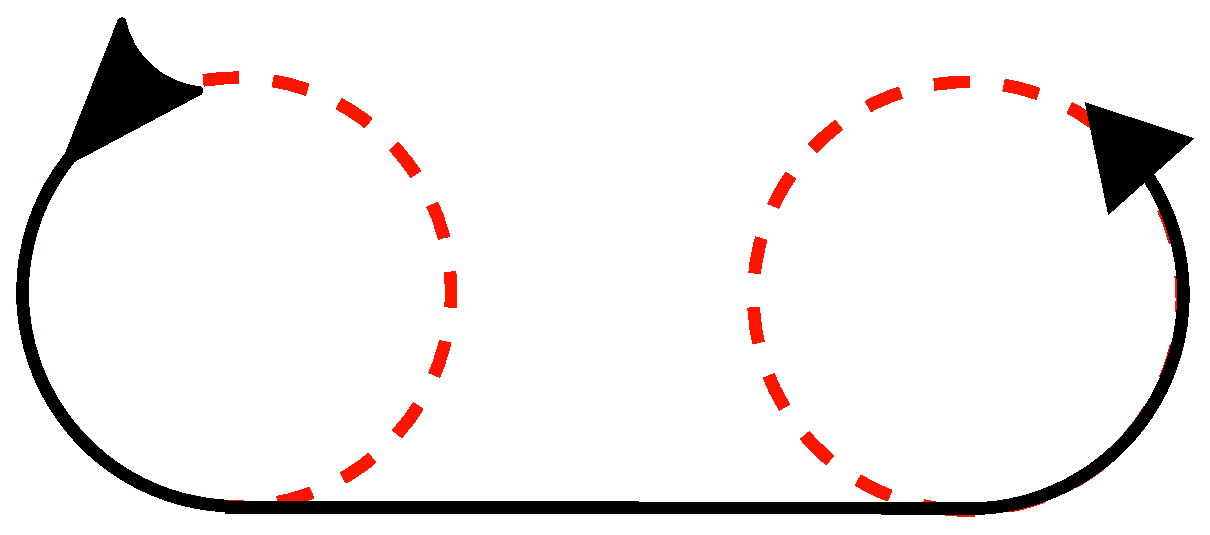
\includegraphics[width=0.5\textwidth]{LSL}
\caption[Dubins LSL Path]{An example LSL Dubins path}
\label{fig:lsl}
\end{figure}

\begin{figure}[htbp!] 
\centering    
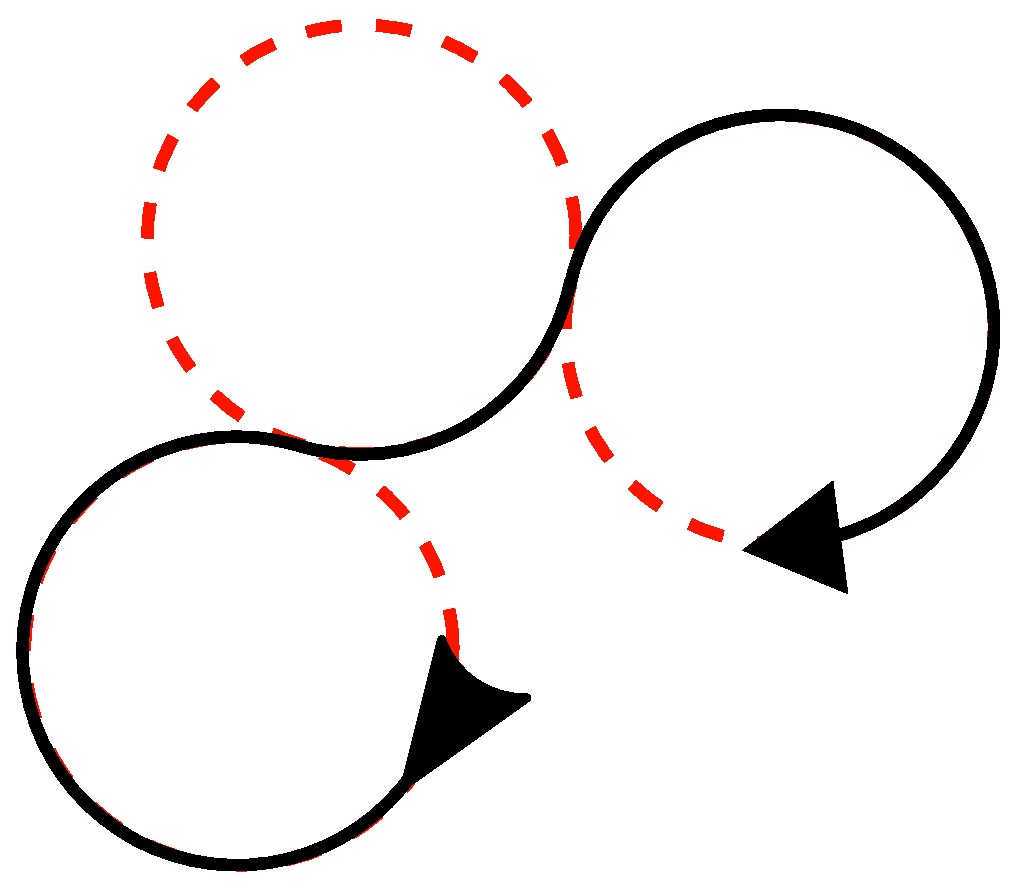
\includegraphics[width=0.5\textwidth]{RLR}
\caption[Dubins RLR Path]{An example RLR Dubins path}
\label{fig:rlr}
\end{figure}

\begin{figure}[htbp!] 
\centering    
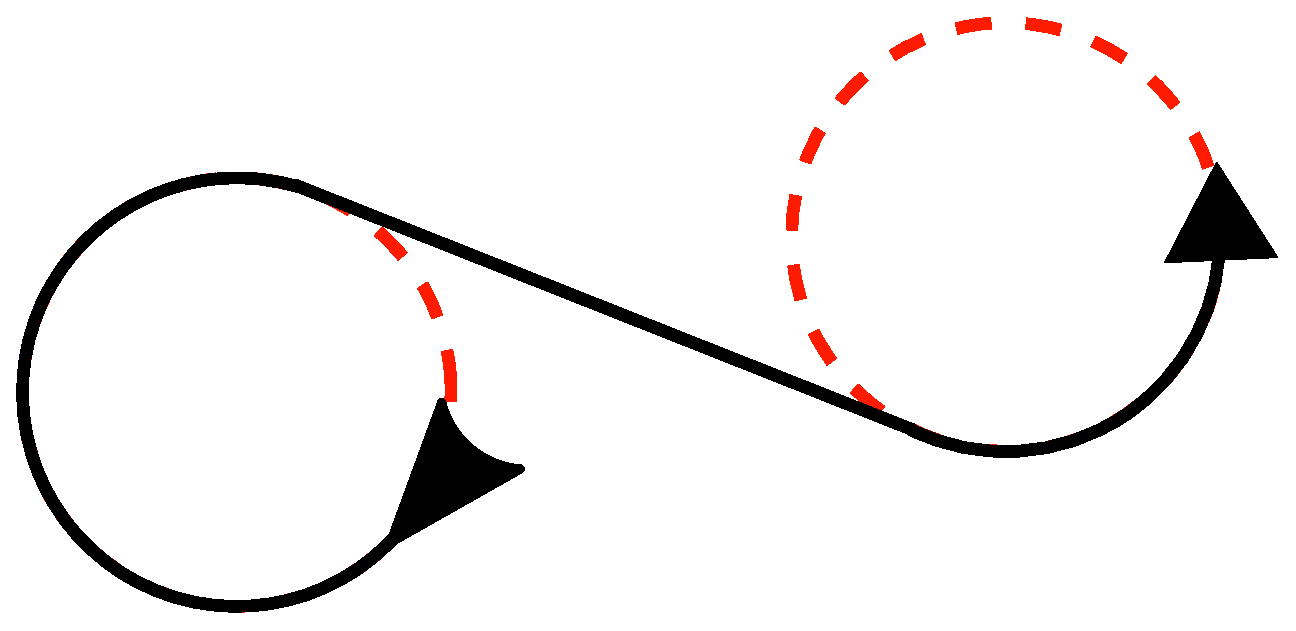
\includegraphics[width=0.5\textwidth]{RSL}
\caption[Dubins RSL Path]{An example RSL Dubins path}
\label{fig:rsl}
\end{figure}

In these diagrams, the arrows show us the initial and final locations, orientations, and direction of travel. The dashed circle in red shows the maximum curvature of any part of the path, which corresponds to a UAV's minumum turning radius. Dubins paths can take many forms, these three examples are intended to enable the reader to visualise their general form and how they relate to the conditions defined above.

Using the notation found in \cite{shkel2001classification}, we can define a paths length as

\begin{equation}
	L = t + p + q
\end{equation}

where $t$, $p$, and $q$ denote the length of the first, second, and third segments respectively \cite{dubins1957curves}. When discussing multiple solutions for the same input parameters, we use subscripts to specify which path we are talking about, for example the length of a given LSL path can be written as

\begin{equation}
	L_{lsl} = t_{lsl} + p_{lsl} + q_{lsl}
\end{equation}

The full set of formulae for calculating the values of $t$, $p$, and $q$ for each path type can be found in \cite{shkel2001classification}. Using this information, we can create a system to evaluate the length of each path type for a given set of input parameters then compare these values with one another to find the shortest path type. The input parameters for this system would be:

\begin{itemize}
	\item The co-ordinates of the start location
	\item The heading at the start location
	\item The co-ordinates of the end location
	\item The heading at the end location
	\item The minimum turning rate of our UAV
\end{itemize}

As these Dubins paths are only operating in one plane, we shall not be enabling these turns to be used to change altitude, and shall calculate our paths assuming the altitude is constant. In this regard, we are only considering paths in the $xy$ plane, and not planning to change altitude in the $z$ plane. 

We can simplify our input parameter set by combining the location and orientation at each end of the path into a single input. We shall use $q_n$ as notation for these points, and as such any Dubins path can be considered to be between $q_0$ and $q_1$. We can define a path end point as 

\begin{equation}
q_n = (x,y,\phi)
\end{equation}

Where $x$ and $y$ are co-ordinates in the $xy$ plane, and $\phi$ is the orientation at this point. The notation in this project dictates that $\phi$ is an angle measured in radians, with $2\pi$ being equivalent to due East, $\pi$ being due West, and so on. 

For an example, using the formulae described in \cite{shkel2001classification} alongside our notation, a Dubins path from

\begin{equation}
q_0 = (0,0,0)
\end{equation}

to

\begin{equation}
q_1 = (10,10,\pi)
\end{equation}

describes a start point facing due East, and an endpoint facing due West which is $\sqrt{10^2 + 10^2}$ units to the North-East of the start location. In this scenario let us assume we are working in metres. If this route is to be flown by a UAV with a minimum turning radius of 20 metres would result in a $LRL$ Dubins path where

\begin{equation}
t = 108.8m 
\end{equation}
\begin{equation}
p = 16.2m 
\end{equation}
\begin{equation}
q = 95.9m 
\end{equation}

Using all of this information, we can find the shortest path from any point in the $xy$ plane to another point in the $xy$ plane, with defined orientations. This is useful for the work in this project as we are ensuring that we use the minimum battery power, completing the turns quickly, and are aligning the UAV with the imaging paths. This last point is important as it provides a means to ensure high quality aerial photographs, as defined in Section \ref{intro:obj1}. Ensuring that the UAV is aligned with an imaging path prior to traversing it means that we can confidently say that once on the imaging path, the images captured will be useful. This simplifies the path planning process as it means no extra steps need to be taken to ensure we are able to capture useful images from the very beginning of the imaging path.

A small standalone application is publicly available and licensed for re-use on GitHub which is capable of calculating the lengths of each type of Dubins path for a given set of input parameters \cite{WalkerDubinsCurves}. This application implements the formulae described in \cite{shkel2001classification} for calculating the lengths of each of these paths, and then returns the values of the shortest path along with its path type. The code for this application is written in C, although a Python version is also available. Extending on this, a MATLAB Mex wrapper is available on the MATLAB MathWorks File Exchange \cite{MexDubinsCurves}, which is a simple C++ wrapper enabling the original application to be imported into MATLAB.

%TODO finalise section

%******************************************************************************************************
%******************************************************************************************************
\section{Paths in Wind}
\label{litrev:path}

One of the most important factors we need to account for at all stages of this project is the effect of wind; we need to be able to account for it in both path planning and path following. The literature discussed in Section \ref{litrev:dubins} is sufficient to enable us to calculate and plan a suitable flight path, only in an environment with zero wind. As such we need to be able to account for the effects of wind in any given direction to still plan a path that will be as short as possible whilst still resulting in the UAV navigating to the correct location.

When considering the effects of wind, it is important to define two frames of reference that shall be in use throughout this paper. The first is what shall be known as the ``ground relative'' frame of reference, and the second is the ``air relative'' frame of reference. The ground relative frame refers to the position of the UAV in relation to the ground, whilst the air relative frame refers to the position of the UAV relative the body of air it is moving through. For this project we shall be treating the air as a consistent fluid that moves at the speed of the wind, relative to the ground. The true and accurate motion of the air is far too complex and out of scope for this project, so the movement of air due to thermal effects and such will not be considered. 

Both frames of reference are considered to be seen from a top-down perspective, as if we were looking directly down on the UAV flying over the ground beneath. This is because ArduPilot defines a mission using waypoints specified by GPS locations, and the flight simulator discussed in Section \ref{intro:jsbsim} also provides this view. In both frames of reference, paths are defined irrespective of any roll, pith, or yaw the UAV may display. For the ground relative frame, it can be best described as the tracking the location of the UAV according to its GPS readings, and for the air relative frame as the movement of the centre of gravity of the UAV through the air. 

We can say that when there is no wind and we treat the air as completely stationary, a ground relative path travelled by the UAV will be the same as the corresponding air relative path. This means that in a zero wind condition we can simply use the formulae discussed above in Section \ref{litrev:dubins} to plan our desired turns, completed using Dubins paths, between imaging paths. Extending on this however, a method for calculating a Dubins path that accounts for the effects of a constant wind is proposed in \cite{mcgee2005optimal}.

This paper proposes a solution that utilises a virtual target point, $vt$, for the UAV to fly to in order to reach our desired location. As we are using our UAV for aerial photography, we are most interested in the commanding the UAV to a location directly above a point on the ground below, as opposed to a location relative to the air. If we define this location on the ground as a location denoted by $d$, its corresponding point in the air relative frame will be moving in the opposite direction to the movement of the air at the same speed as the wind speed. 


Fig. \ref{fig:windalgorithm} shows us how we work out the movement of the virtual target. $q_0$ is the end point of one imaging run, and $d$ is the start of the next imaging run. We need to find a Dubins path between these two points with the correct orientations, accounting for the wind vector shown at the top of the diagram. Both $q_0$ and $d$ are ground relative points, whilst $vt$ is a point relative to the air through which the UAV is travelling. With respect to the air, $vt$ is moving opposite to the wind, and as such tracks the movement of $d$ relative to the air.
\vspace{1cm}
\begin{figure}[htbp!] 
\centering    
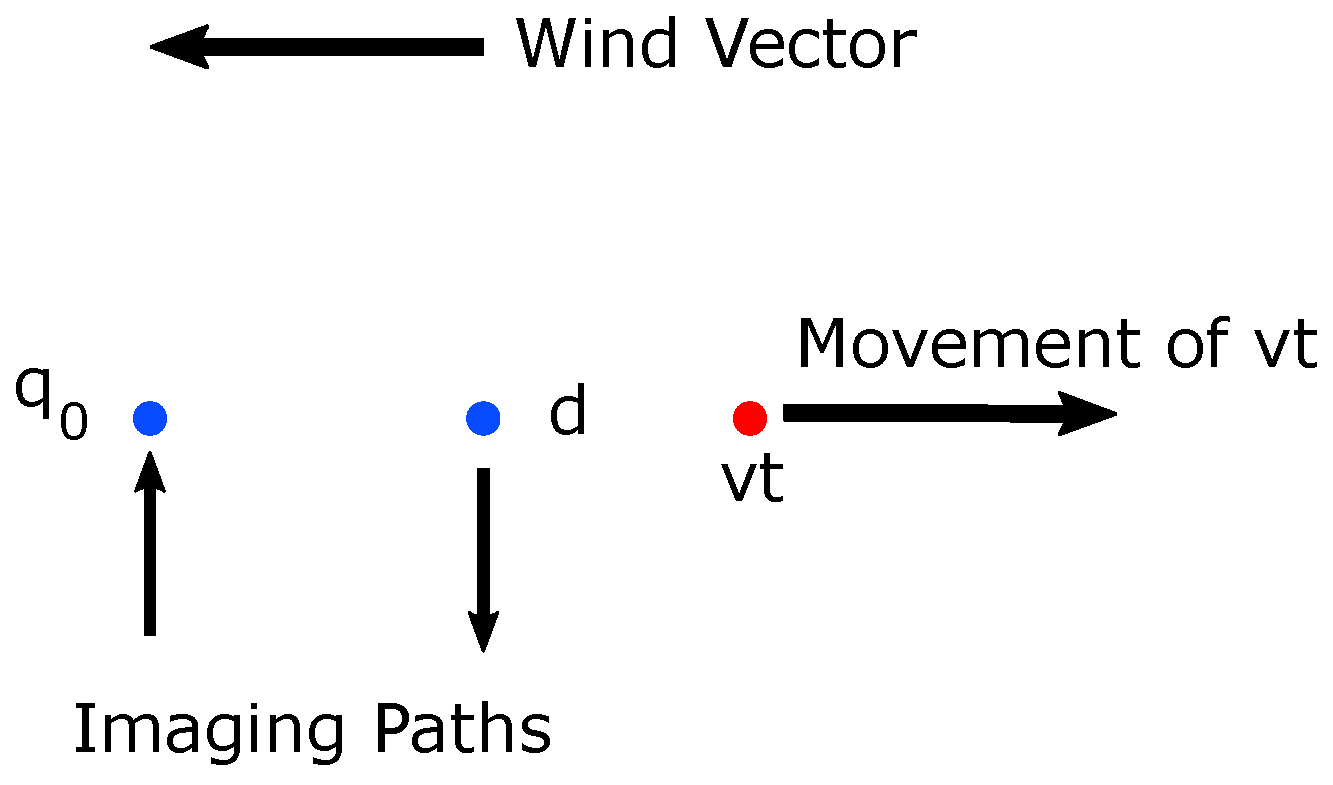
\includegraphics[width=0.7\textwidth]{WindAlgorithm}
\caption[Calculating a Dubins Path in Wind]{A display of how the virtual target point moves with regard to the start and end points of our path and wind}
\label{fig:windalgorithm}
\end{figure}

To find a suitable path, we need to define two time measurements; $T_{vt}$ and $T_a$. $T_{vt}$ is the time taken for the virtual target to have moved from $d$ to its current location, whilst $T_{vt}$ is the time taken for the UAV to fly a Dubins path from $q_0$ to the location of $vt$. To find a solution to this problem, we must find a point at which $T_a$ and $T_{vt}$ are equal, which will result in the UAV flying to the point $vt$ with the desired orientation, and as such be directly over point $d$. 

%TODO explain momentum and heading vectors

We are able to use this information to generate a search algorithm which will find a suitable Dubins path to follow to correctly complete a turn between imaging paths in wind, utilising Dubins path to minimise flight time and battery usage. This technique should, in theory, allow us to calculate suitable paths in any wind condition providing the wind is moving slower than the maximum airspeed of the UAV. It does have major limitations however, in that it assumes constant wind in both speed and direction. %TODO extend downfalls of this method.

Another problem, as discussed in \cite{mcgee2005optimal}, is that for certain scenarios, this search algorithm will fail. This can occur when flying in a very low wind environment, resulting in the $vt$ moving very slowly, whilst the UAV is travelling a lot faster. This will mean that due to the differences in speed, there is no point at which one of the 6 regular Dubins paths will satisfy the condition of $T_a$ and $T_{vt}$ being equal. A solution to this is to fly a non-optimal path, meaning a path which is no longer the shortest between the two points. There are a number of ways to solve this, including adding two new path types based on LRL and RLR paths. These new types can be used to travel a longer $p$ segment of the path, thus lengthening the path in order to provide a solution to the algorithms equality condition. Details on how these paths are calculated can be found in \cite{mcgee2005optimal}. %TODO explain LRL outer and inner etc?

%TODO define vt intercept
%TODO summarise section to round it off
%TODO define cross track error

%******************************************************************************************************
%******************************************************************************************************
\section{ArduPlane Documentation}
\label{litrev:arduplane}

As the entire ArduPilot project is open source and not run in an effort to generate revenue, there is little incentive for its developers to maintain thorough documentation or to extend support for old versions of their products. There are however a number of articles available on the ArduPilot developer wiki, which is a subsection of their main website \cite{ArduPilotDev}. Important resources include
\begin{itemize}
  	\item Use of SITL utilizing JSBSim: \url{http://ardupilot.org/dev/docs/using-sitl-for-ardupilot-testing.html}
  	\item How to add a new flight mode to ArduCopter: \url{http://ardupilot.org/dev/docs/apmcopter-adding-a-new-flight-mode.html}
  	\item How to add new navigation commands: \url{http://ardupilot.org/dev/docs/code-overview-adding-a-new-mavlink-message.html}
  	\item How to build the code using various techniques on a number of operating systems: \url{http://ardupilot.org/dev/docs/building-the-code.html}
  \end{itemize}  

These wiki pages are very useful in starting to understand the code, however often are specific to the newest ArduPilot versions and are sometimes even specific to ArduCopter, as this appears to be the most popular of their products. 

Outside of this developer wiki, the only other useful information comes from other users and developers of the code. This information is found on two forums

\begin{itemize}
	\item The diydrones user forums: \url{http://diydrones.com/forum}
	\item The official ArduPilot forums: \url{http://discuss.ardupilot.org/}
\end{itemize}

Gathering information from these two forums can be rather tedious, as the search functions on the diydrones forum is weak, and finding results depends on either asking a question or someone having already asked it in the past (many of which may not have even received an answer). 

%TODO finalise arduplane nonsense